\documentclass[11pt]{article}

\usepackage[utf8]{inputenc} % character encoding - you don't need to understand this

% Note that if you want to make a number sign, you need to type \#
% below are a bunch of useful packages, it doesn't cost anything to include them all so you might as well
\usepackage{amsmath}		            % lets you input equations in math mode
\usepackage{graphicx}		            % lets you include images
\usepackage{enumerate}		            % lets you make lists
\usepackage{subcaption}                 % if you want to use subcaptions
\usepackage[colorlinks=true]{hyperref}  % for making hyperlinks
\usepackage{hypcap}	                    % makes links refer to figures and not captions
\usepackage{relsize}		            % lets you use relative font sizes
\usepackage{caption}                    % lets you add captions
\usepackage{array}                      % lets you specify table column widths
\usepackage[margin=1in, paperwidth=8.5in, paperheight=11in]{geometry}
\usepackage{listings}
\usepackage{float}
\usepackage{tabularx}
\usepackage{textgreek}
\usepackage{amssymb}
\usepackage{amsthm}
\usepackage{placeins}
\usepackage{imakeidx}
\renewcommand{\qedsymbol}{$\blacksquare$}
\usepackage{blindtext}
\usepackage{csquotes}
\usepackage{pdfpages}
\usepackage[style=numeric-comp,sorting=none]{biblatex}
% \usepackage{biblatex}
\addbibresource{thesis.bib}
\makeindex[columns=2, title=Alphabetical Index, 
options= -s example_style.ist, intoc]

% Note that if you want to make a number sign, you need to type \#
\hypersetup{
    colorlinks=true,
    linkcolor=blue,
    filecolor=magenta,
    urlcolor=cyan,
}

\lstdefinestyle{mystyle}{
  backgroundcolor=\color{backcolour},   commentstyle=\color{codegreen},
  keywordstyle=\color{magenta},
  numberstyle=\tiny\color{codegray},
  stringstyle=\color{codepurple},
  basicstyle=\ttfamily\footnotesize,
  breakatwhitespace=false,         
  breaklines=true,                 
  captionpos=b,                    
  keepspaces=true,                 
  numbers=left,                    
  numbersep=5pt,                  
  showspaces=false,                
  showstringspaces=false,
  showtabs=false,                  
  tabsize=2
}

\begin{document}
\title{Mixed Analog-Digital VLSI Mini-Project III: Folded Cascode Differential Amplifier}
\author{Qingmu Deng}
\maketitle % this line makes the title appear, along with today's date, automatically updated.

\tableofcontents

\section*{Project Links}

Project Github: \href{https://github.com/QingmuDeng/MADVLSI/tree/main/mini2}{https://github.com/QingmuDeng/MADVLSI/tree/main/mini2}

\section{Circuit Analysis and Bias Voltage Generation}
    \subsection{Question a}
        $V_1$ is the non-inverting input while $V_2$ is the inverting input.
        \begin{figure}[!ht]
            \centering
            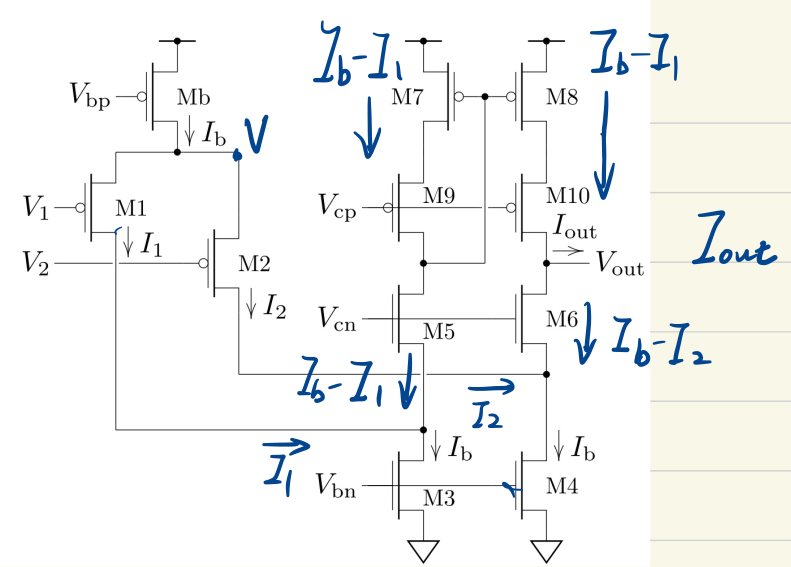
\includegraphics[width=.5\linewidth]{../img/qa.png}
            \caption{Illustration of current flow in folded-cascode differential amplifier for Question a.}
            \label{fig:qa}
        \end{figure}

        This result can be reasoned as the following in conjunction with Figure \ref{fig:qa}. M$_b$ acts as if like a current source to dump $I_b$ into the node $V$. By Kirchoff's current law, the current through M$_1$ and M$_2$ must be in such a way that $I_b=I_1+I_2$. Now let's examine the drain of the transistor M$_3$. At this node, the current coming from M$_1$ is $I_1$, and the current flowing through M$_3$ is $I_b$. By Kirchoff's current law, the current $I_5$ flowing into this node from M$_5$ must be $I_b-I_1$. Assuming all the cascode transistors are bias properly, this current will be mirrored to $I_b-I_2$ flowing into node $V_{out}$ from M$_10$. By the same token, the current $I_6$ flowing out of $V_{out}$ into M$_6$ must be $I_b-I_2$. By Kirchoff's current law, $I_{out}=I_b-I_1-I_b+I_2=I_2-I_1$.

        As we increase $V_2$ while holding $V_1$ fixed, $I_2$ decreases whereas $I_1$ increases. Thus, $I_2-I_1$ decreases. On the other hand, as we increase $V_1$ while holding $V_2$ fixed, $I_1$ decreases whereas $I_2$ increases. Thus, $I_2-I_1$ increases. Therefore, $V_1$ is the non-inverting input, and $V_2$ is the inverting input. 
    \subsection{Question b}
        \begin{figure}[!ht]
            \centering
            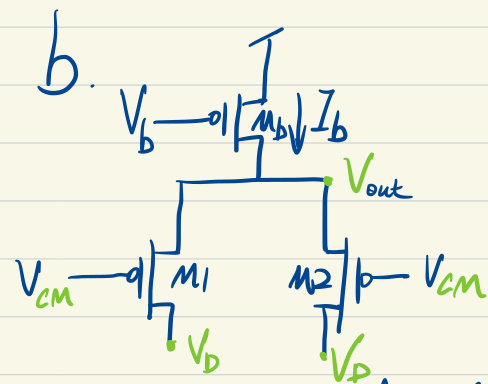
\includegraphics[width=.5\linewidth]{../img/qb.png}
            \caption{Illustration of differential pair for Question b.}
            \label{fig:qb}
        \end{figure}
    To understand the limit on the common-mode input voltage, we treat the differential pair, M$_1$ and M$_2$, and their bias transistor, M$_b$, as a source-follower. For M$_b$ to act like a current source, it must remain in saturation. That is, $I=I_F+I_R\approx I_F$. Thus, we can describe our transistor operation with only the forward current of the source-drain-symmetric EKV model for the transistor operation.
    \begin{equation}
        I_b = SI_s\log^2\Big(1+e^{[\kappa(V_{dd}-V_b)-V_{T_0}-V_{dd}+V_{dd}]/2U_T}\Big)
    \end{equation}
    Similarly, for either M$_1$ or M$_2$, we have
    \begin{equation}
        I_{\text{diff}} = SI_s\log^2\Big(1+e^{[\kappa(V_{dd}-V_{cm})-V_{T_0}-V_{dd}+V_{out}]/2U_T}\Big)
    \end{equation}
    Setting the two equation equal and cancelling terms, we get
    \begin{align}
        I_b&=I_{\text{diff}}\nonumber\\
        \kappa(V_{dd}-V_{cm})-V_{T_0}-V_{dd}+V_{out}&=\kappa(V_{dd}-V_b)-V_{T_0}\nonumber\\
        V_{dd}-V_{out}&=\kappa(V_{dd}-V_{cm}-V_{dd}+V_b)\nonumber\\
        V_{out} &= V_{dd} - \kappa(V_b-V_{cm})
    \end{align}
    At the same time, we know that for M$_b$ to be in saturation, its source-drain voltage must be at least a certain $V_{SDSAT}$.
    \begin{align}
        V_{dd} - V_{out} \geq V_{SDSAT}\nonumber\\
        V_b - V_{cm} \geq V_{SDSAT}/\kappa\nonumber\\
        V_{cm} \leq V_b - V_{SDSAT}/\kappa
    \end{align}
    
    \subsection{Question c}
    If the output node is held fixed near the middle of the rails and the Early effect is negligible, the output current is given by
    \begin{equation}
        I_{out}=I_b-I_1-I_b+I_2=I_2-I_1
    \end{equation}
    For its derivation, see answer to Question a.
    
    \subsection{Question d}
    The current at the bias transistors M$_3$ and M$_4$ need not be biased to exactly $I_b$ as in the bias transistor M$_b$. However, two constraints exist:
    \begin{enumerate}
        \item The bias current in M$_3$, $I_{b3}$, and the bias current in M$_4$, $I_{b4}$, must be equal to each other. Their equal current nature is necessary for their cancellation in the output current of the $V_{out}$ node. Otherwise, there will be a constant term in output current that is not directly to either of the input voltages.
        \item The bias current in both M$_3$ and M$_4$ must be at least $I_b$ or larger. The current through M$_5$ and M$_6$ is given by $I_5=I_{b3}-I_1$ and $I_6=I_{b4}-I_2$, respectively. In situations where $I_1=I_b,\ I_2=0$, for example, we have $I_5=I_{b3}-I_b<0$ and $I_6=I_{b4}$. This is problematic as it seems to suggest that the current should flow into the pmos current mirror from the nmos instead of the other way around. What could realistically happen is that the current $I_1$ drives the drain voltage of M$_3$ so high such that it is passing through $I_b$ equivalent amount of current through Early effect.
    \end{enumerate}

    \subsection{Question e}
    The bias voltage generation circuit is designed as shown in Figure \ref{fig:biasgen}. A diode-connected unit nmos accepts the current and have it mirrored to a group of bias voltage generation transistors for either pmos or nmos.
    \begin{figure}[!ht]
        \centering
        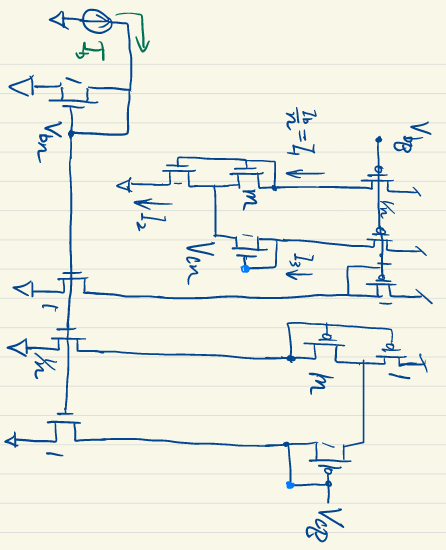
\includegraphics[width=.5\linewidth, angle=90]{../img/biasgen.png}
        \caption{Cascode-bias voltage generation circuit design.}
        \label{fig:biasgen}
    \end{figure}
    The group of bias-voltage generation transistors for $V_{cn}$ generation can be laid out in the way shown in Figure \ref{fig:cn_design}, and the group of bias-voltage generation transistor for $V_{cp}$ generation is similarly shown in Figure \ref{fig:cp_design}.
    \begin{figure}[!ht]
        \centering
        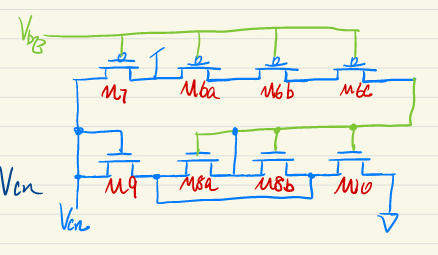
\includegraphics[width=.5\linewidth]{../img/cn_design.png}
        \caption{$V_{cn}$ voltage generation circuit layout driven schematics.}
        \label{fig:cn_design}
    \end{figure}
    \begin{figure}[!ht]
        \centering
        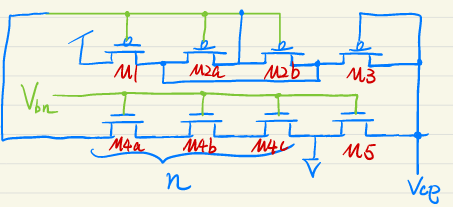
\includegraphics[width=.5\linewidth]{../img/cp_design.png}
        \caption{$V_{cp}$ voltage generation circuit layout driven schematics.}
        \label{fig:cp_design}
    \end{figure}

    To achieve the common centroid design, both group of the transistors were mirrored along their edges. The $12\times0.5\mu m$transistor is therefore divided up into two $6times0.5\mu m$ unit transistors. The auxiliary current mirrors forms a standalone block in the layout driven schematic. The schematic for the entire folded cascode differential amplifier is shown in Figure \ref{fig:schem_all}.

    \begin{figure}[!ht]
        \centering
        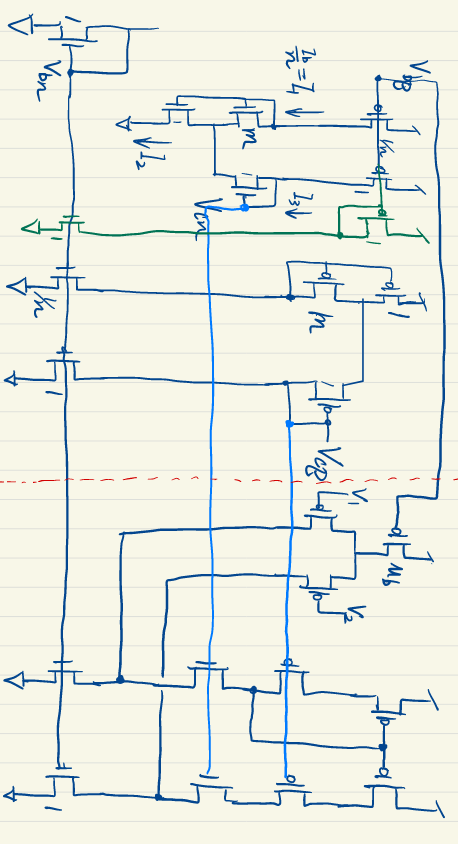
\includegraphics[width=.5\linewidth, angle=90]{../img/schem_all.png}
        \caption{The circuit design for the entire folded cascode differential amplifier with bias voltage generation.}
        \label{fig:schem_all}
    \end{figure}



\section{Schematic Capture and Simulation}
    \subsection{Schematic Capture}
    The layout driven schematics for both the cascode bias generation circuit and the folded cascode differential amplifier is created separately, as shown in Figure \ref{fig:bias_schm} and \ref{fig:cas_schm}. Both circuits independently adopt a common centroid configuration. All the bias and cascode transistors were all matched to Size $6\mu m \times 0.5\mu m$ and combined in series and in parallel to ultimately achieve the effective size of $12\mu m \times 0.5\mu m$. The differential pair were matched to each other through series and parallel combinations of Size $12\mu m \times 0.5\mu m$. Appropriately sized dummy transistors have been added to the end of transistor rows wherever applicable.
    
    \begin{figure}[!ht]
        \centering
        \begin{subfigure}{\linewidth}
            \centering
            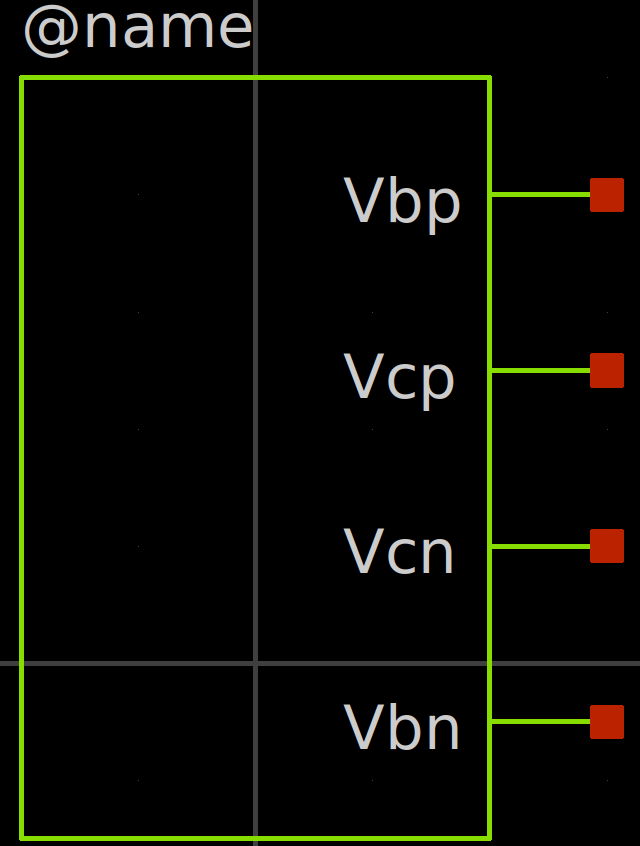
\includegraphics[width=0.2\linewidth]{../img/bias_sym.png}
            \caption{Cascode bias voltage generation symbol created in Xschem.}
        \end{subfigure}\\
        \begin{subfigure}{1.0\linewidth}
            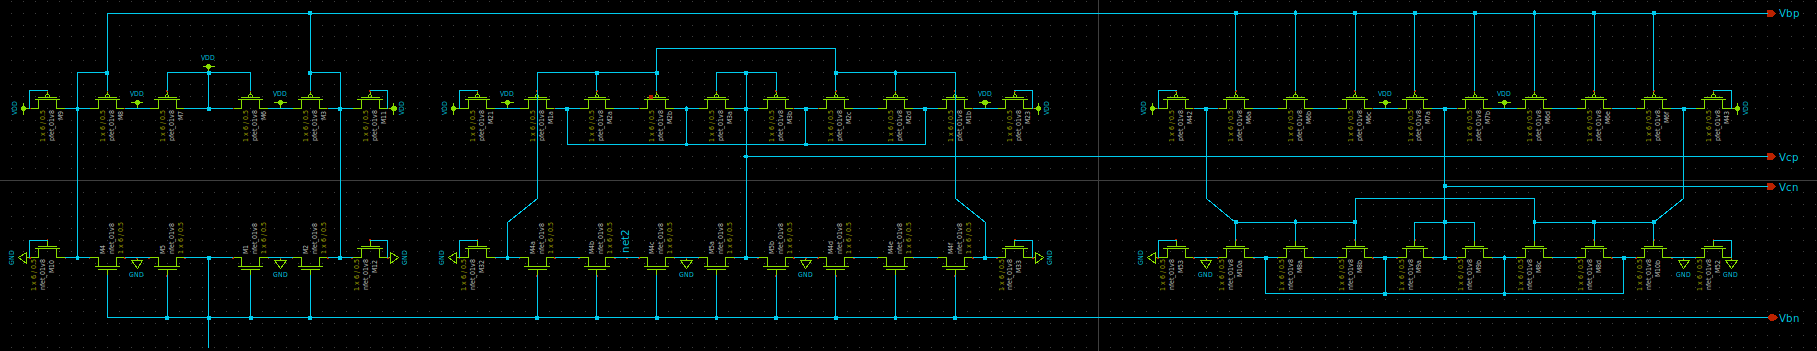
\includegraphics[width=\linewidth]{../img/bias_sch.png}
            \caption{Cascode bias voltage generation layout-driven schematic created in Xschem.}
        \end{subfigure}
        \caption{Cascode bias voltage generation schematic capture in Xschem.}
        \label{fig:bias_schm}
    \end{figure}
    \begin{figure}[!ht]
        \centering
        \begin{subfigure}{\linewidth}
            \centering
            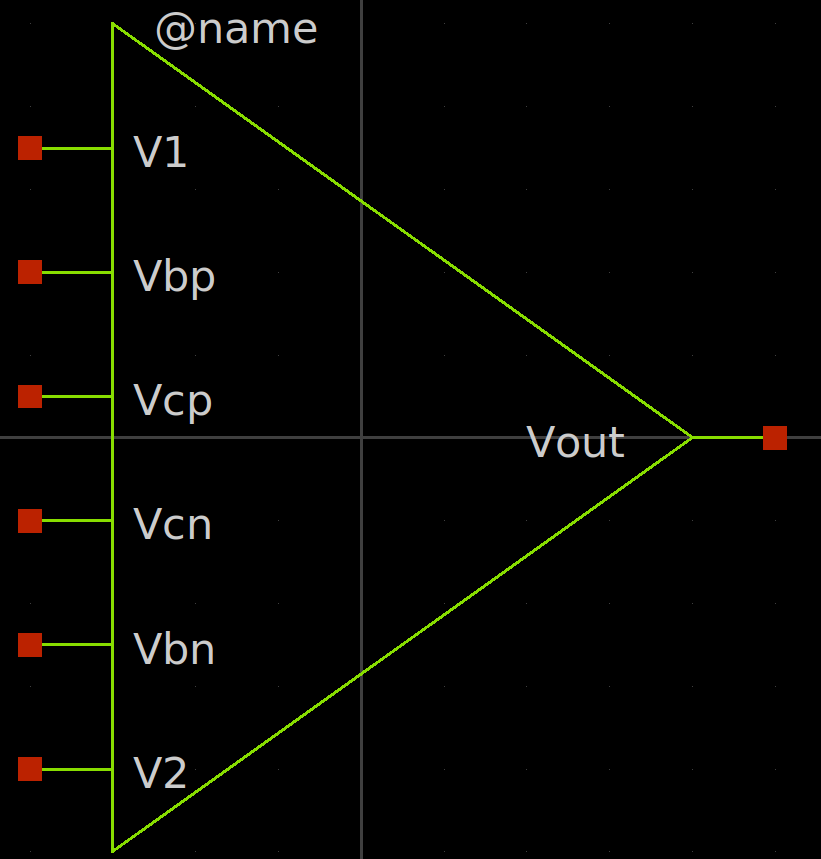
\includegraphics[width=0.2\linewidth]{../img/cas_sym.png}
            \caption{Folded cascode differential amplifier symbol created in Xschem.}
        \end{subfigure}\\
        \begin{subfigure}{1.0\linewidth}
            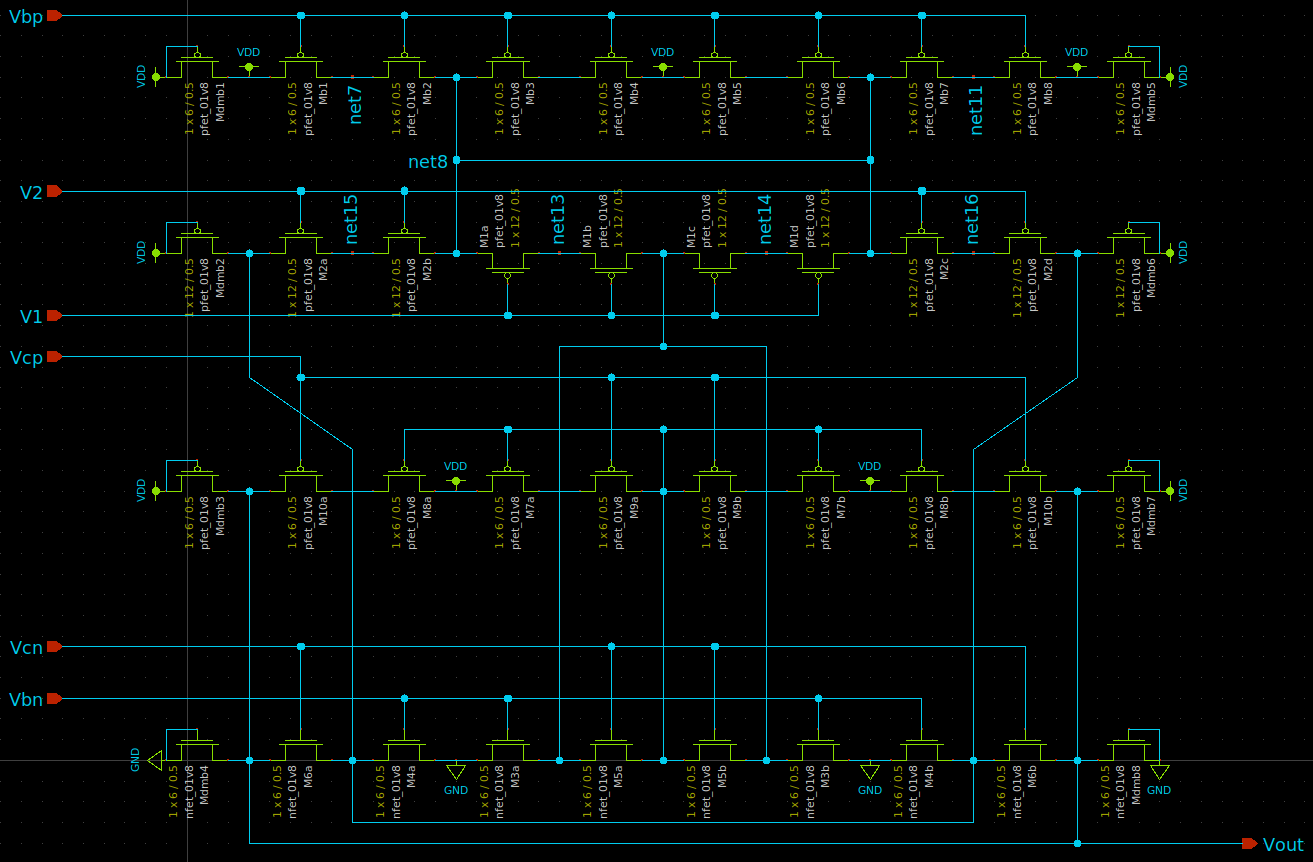
\includegraphics[width=\linewidth]{../img/cas_sch.png}
            \caption{Cascode bias voltage generation layout-driven schematic created in Xschem.}
        \end{subfigure}
        \caption{Folded cascode differential amplifier schematic capture in Xschem.}
        \label{fig:cas_schm}
    \end{figure}

    \subsection{Test Harness}
    For the test harness configuration, please refer to Figure \ref{fig:vtc} to \ref{fig:lsig}. For the simulation results and their interpretations, please refer to Section \ref{sec:res}.
    \begin{figure}[!ht]
        \centering
        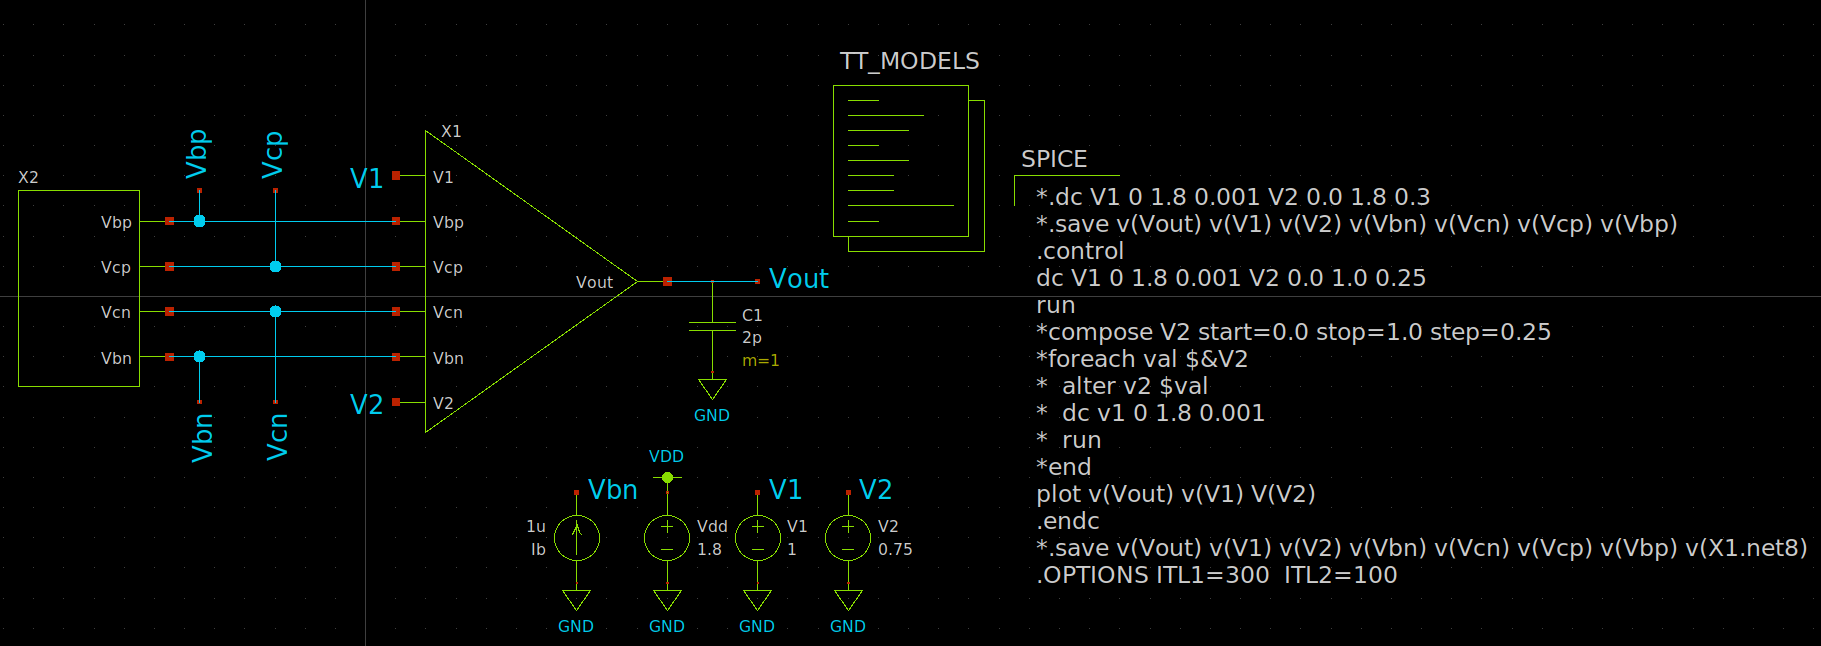
\includegraphics[width=.95\linewidth]{../img/vtc.png}
        \caption{DC voltage transfer characteristics test harness.}
        \label{fig:vtc}
    \end{figure}
    \begin{figure}[!ht]
        \centering
        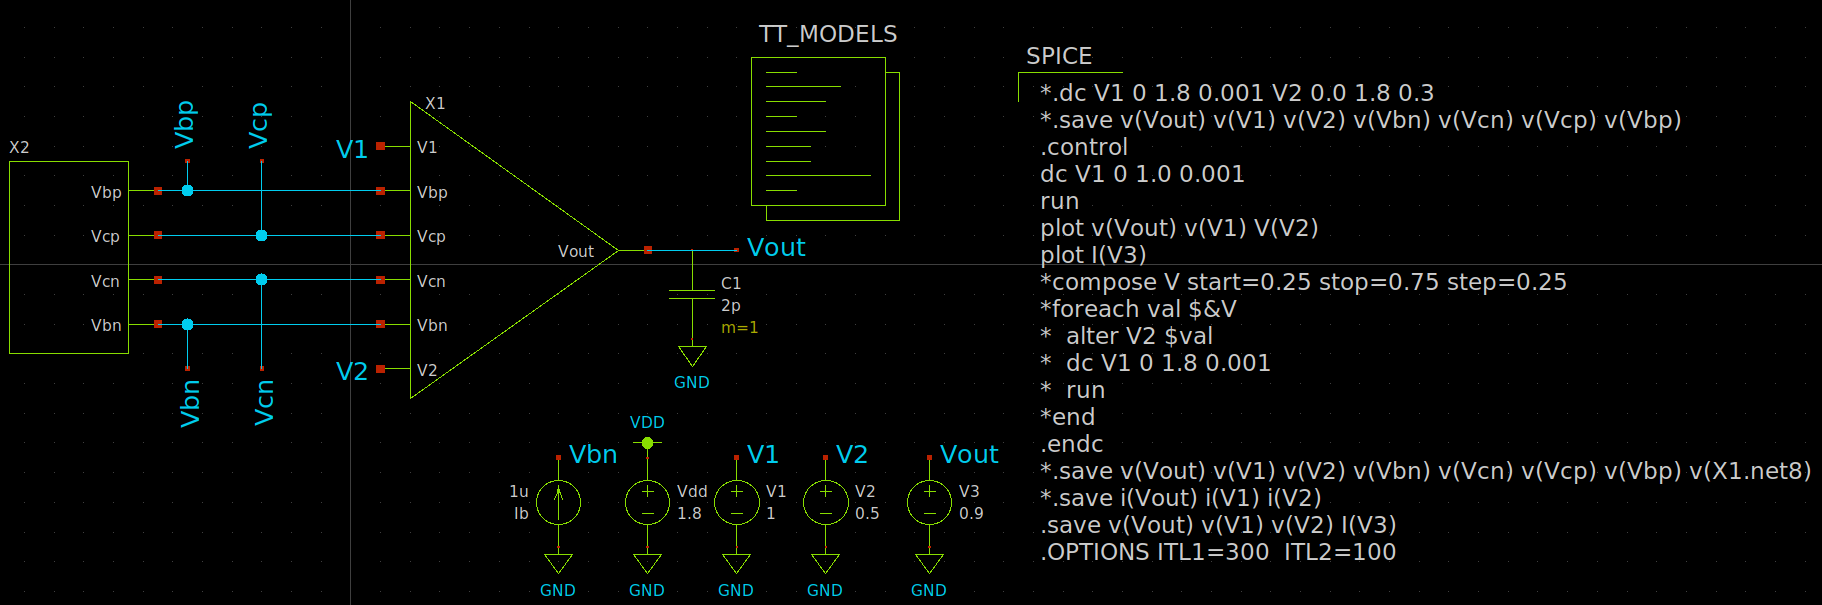
\includegraphics[width=.95\linewidth]{../img/v2i.png}
        \caption{Voltage-to-current transfer characteristics test harness.}
        \label{fig:v2i}
    \end{figure}
    \begin{figure}[!ht]
        \centering
        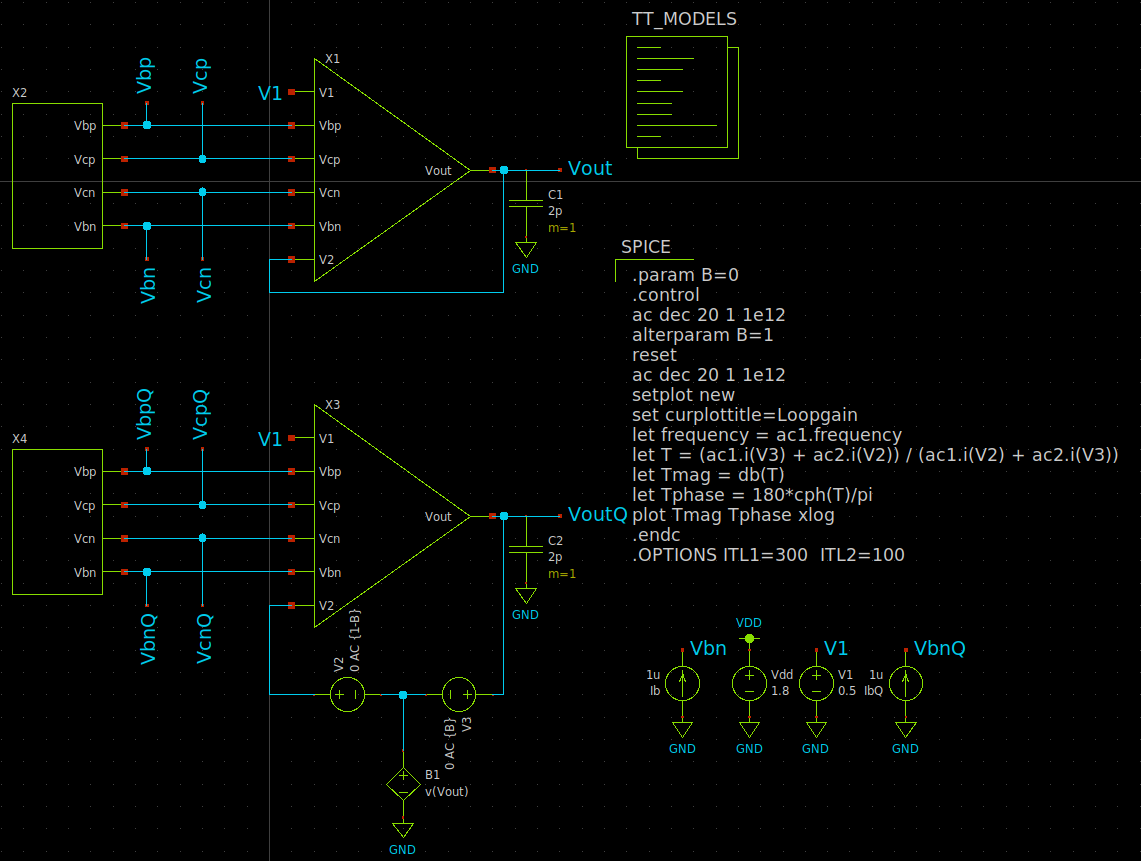
\includegraphics[width=.85\linewidth]{../img/loopgain.png}
        \caption{Loopgain test harness.}
        \label{fig:loopgain}
    \end{figure}
    \begin{figure}[!ht]
        \centering
        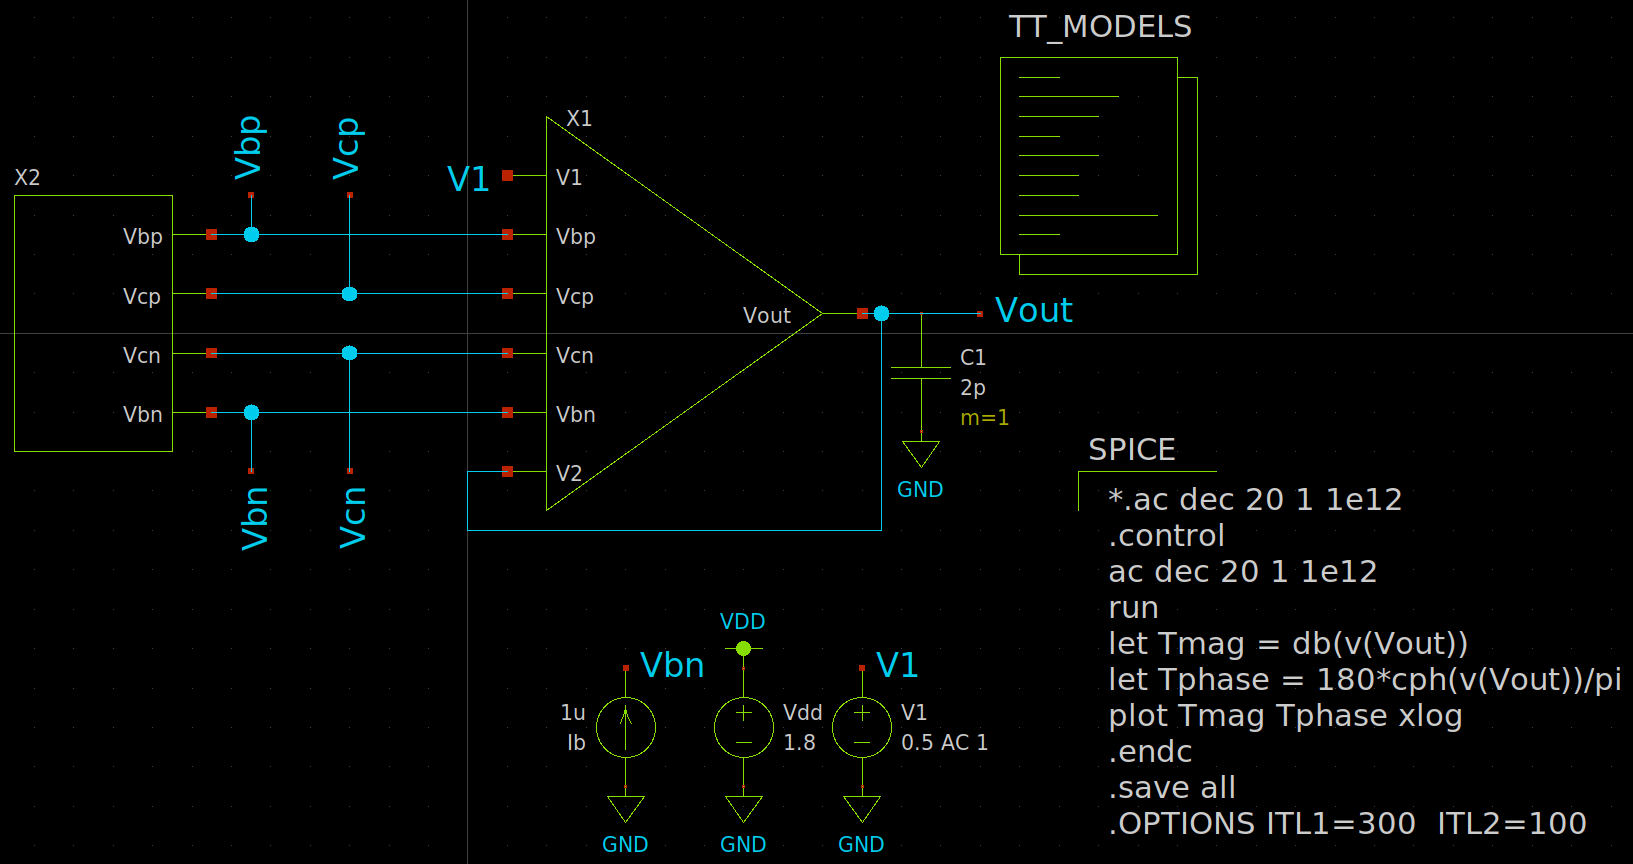
\includegraphics[width=.90\linewidth]{../img/ac.png}
        \caption{Unity-gain follower frequency response test harness.}
        \label{fig:ac}
    \end{figure}
    \begin{figure}[!ht]
        \centering
        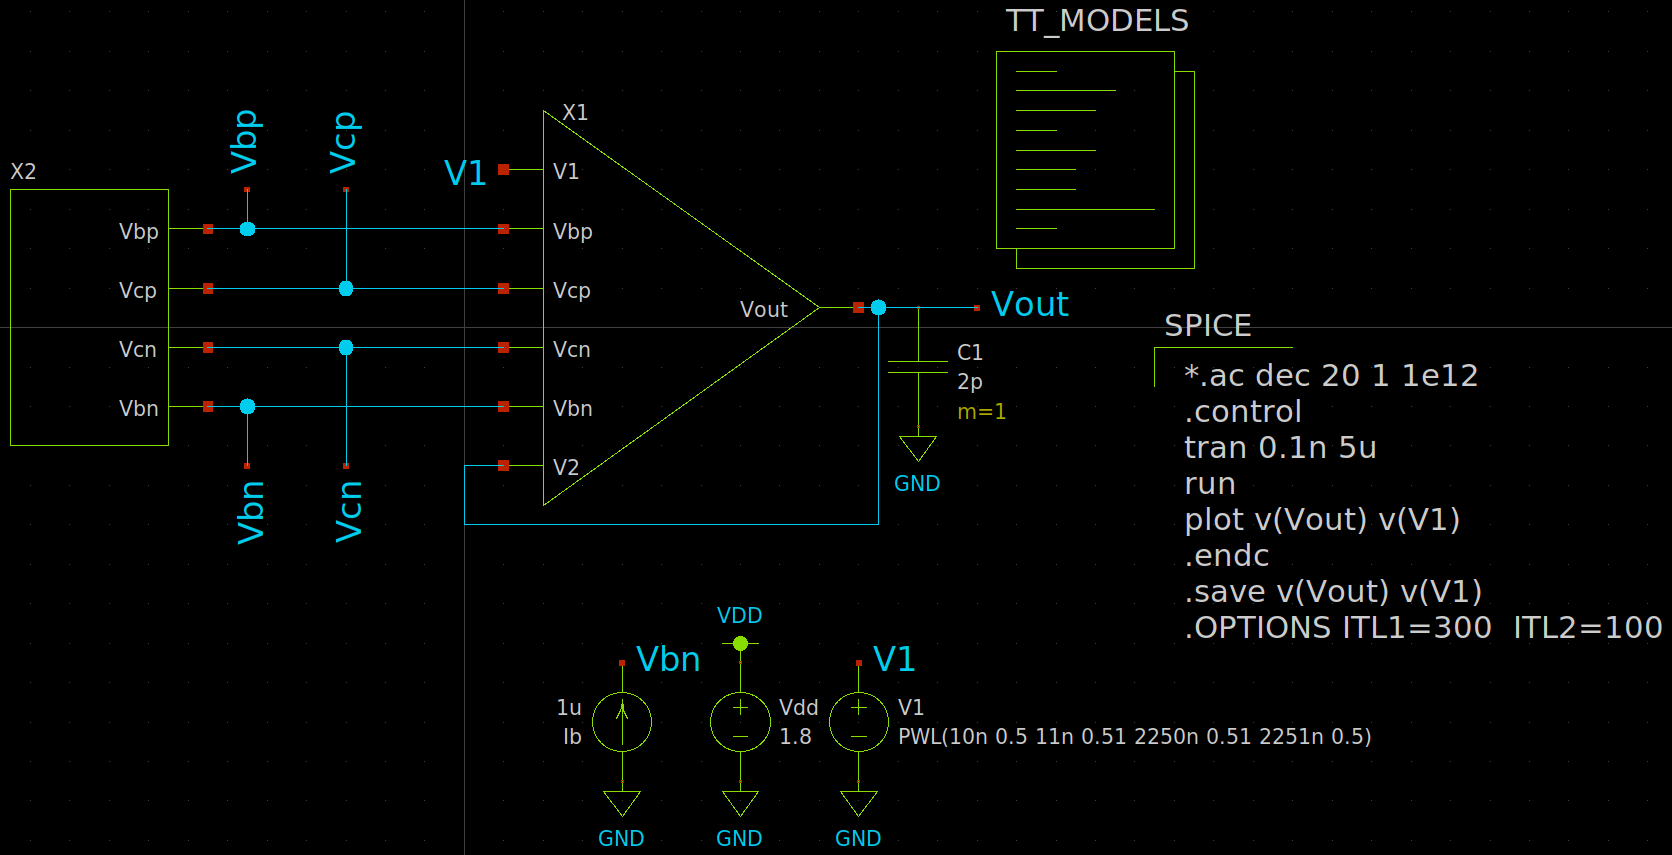
\includegraphics[width=.90\linewidth]{../img/ssig.png}
        \caption{Small signal test harness.}
        \label{fig:ssig}
    \end{figure}
    \begin{figure}[!ht]
        \centering
        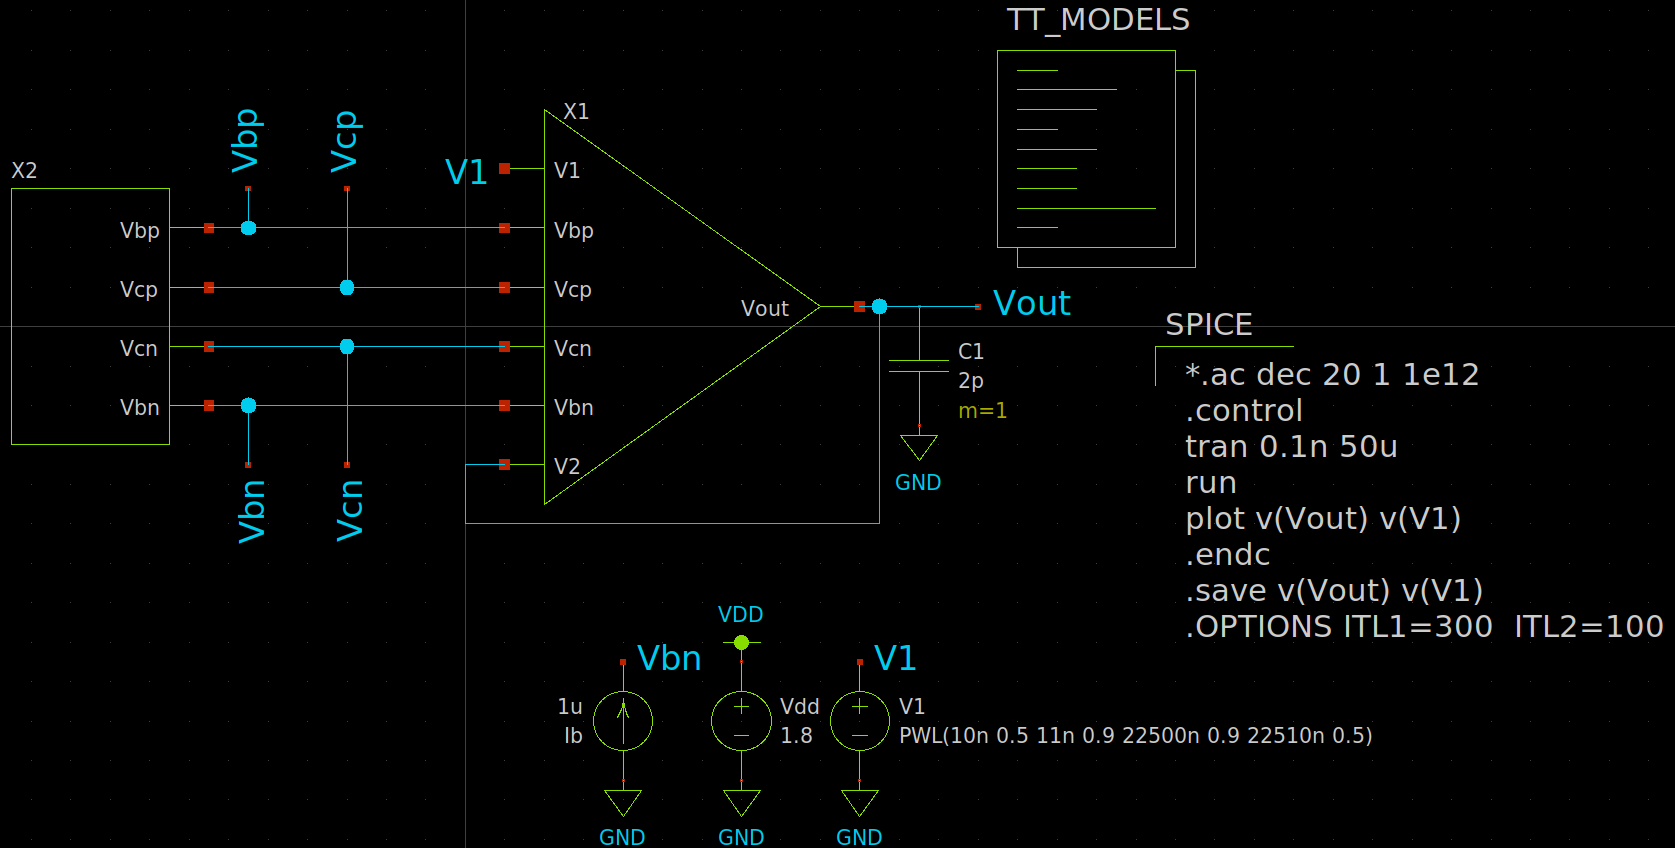
\includegraphics[width=.90\linewidth]{../img/lsig.png}
        \caption{Large signal test harness.}
        \label{fig:lsig}
    \end{figure}
    

\FloatBarrier
\section{Layout Design}
    There are no design rule violations. TAll the bias and cascode transistors were all matched to Size $6\mu m \times 0.5\mu m$ and combined in series and in parallel to ultimately achieve the effective size of $12\mu m \times 0.5\mu m$. The differential pair were matched to each other through series and parallel combinations of Size $12\mu m \times 0.5\mu m$. Appropriately sized dummy transistors have been added to the end of transistor rows wherever applicable.

    The area of the bias circuit is $515.14\ \mu m^2$; the area of the folded cascode differential amplifier is $476\ \mu m^2$.

    \begin{figure}[!ht]
        \centering
        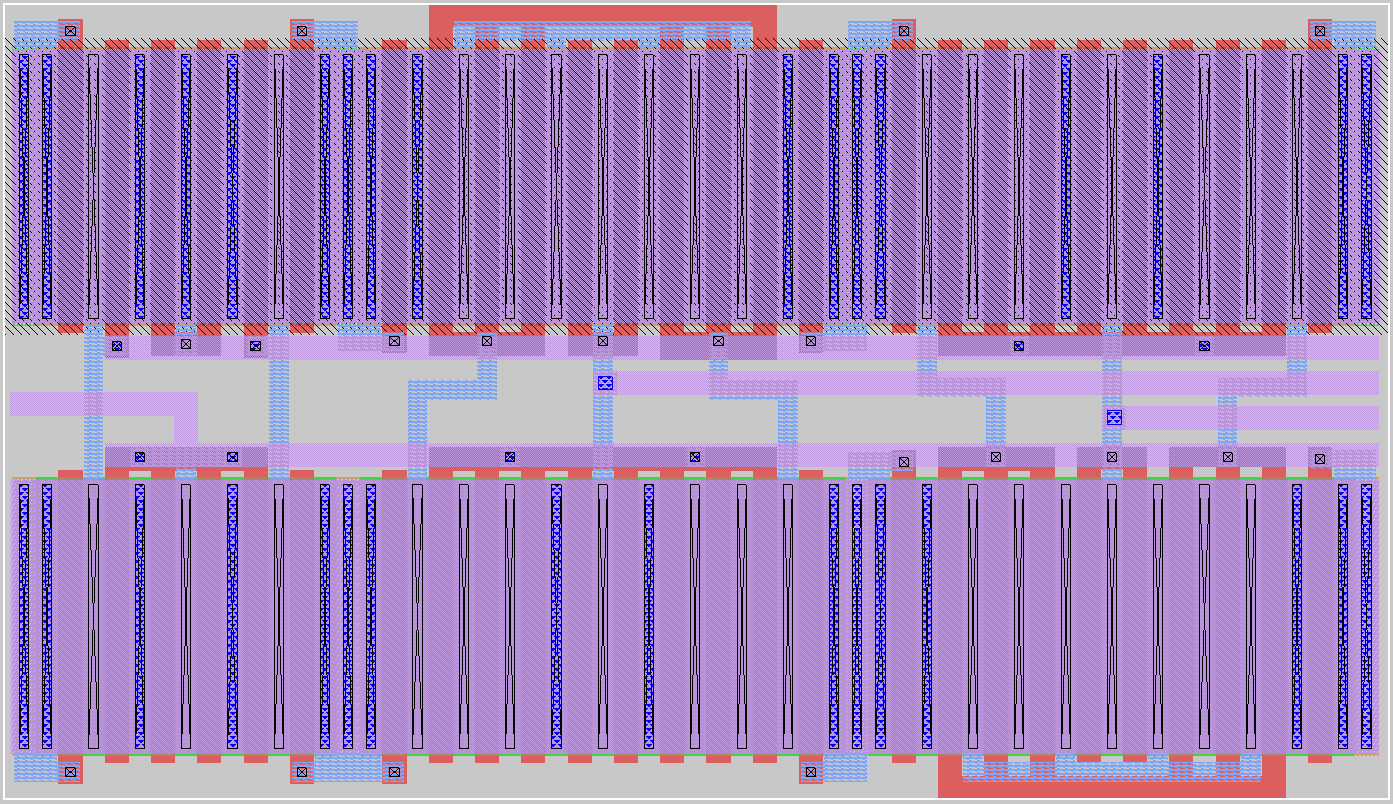
\includegraphics[width=0.99\linewidth]{../img/bias_mag.png}
        \caption{\textit{Magic} layout of the cascode bias voltage generation circuit.}
        \label{fig:biasmag}
    \end{figure}
    \begin{figure}[!ht]
        \centering
        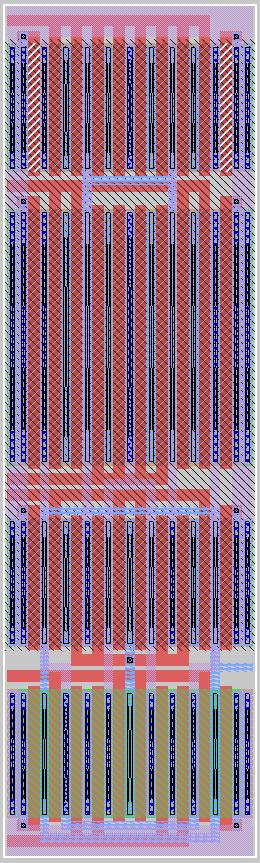
\includegraphics[width=0.4\linewidth]{../img/cas_mag.png}
        \caption{\textit{Magic} layout of the Folded cascode differential amplifier.}
        \label{fig:casmag}
    \end{figure}
    \begin{figure}[!ht]
        \centering
        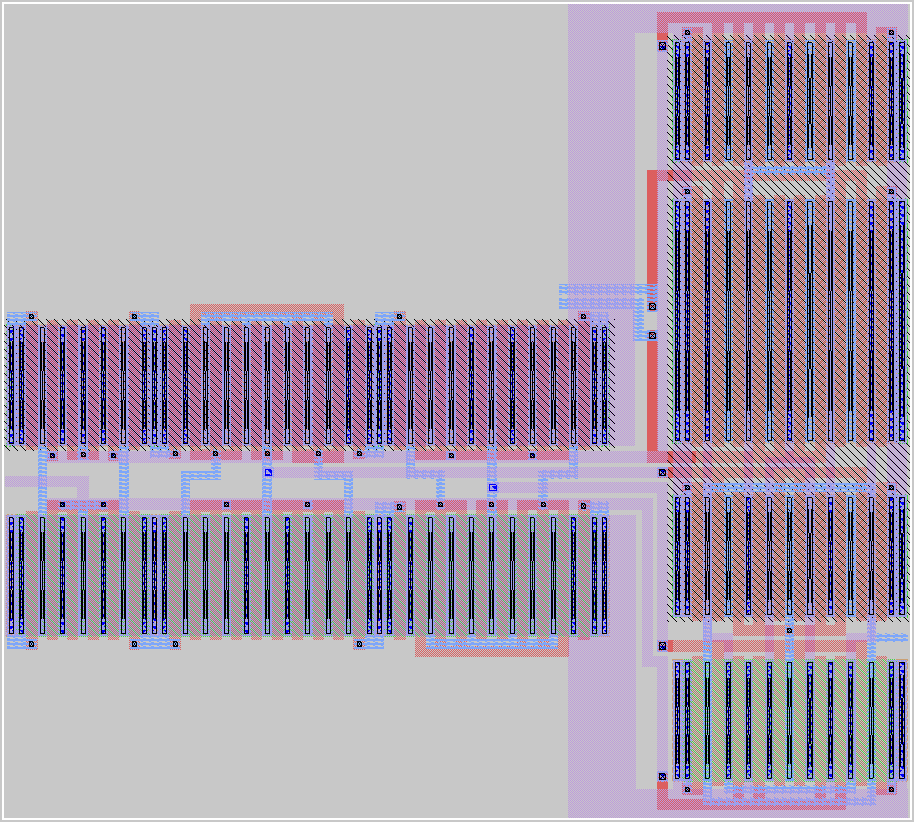
\includegraphics[width=1.1\linewidth, angle=-90]{../img/joint_mag.png}
        \caption{Joining the two layouts in \textit{Magic}.}
        \label{fig:joitmag}
    \end{figure}
    \FloatBarrier
    \section{Layout versus Schematic}
    Finally, I performed Layout-versus-Schematic comparison at all levels of the shift register. There are three listings below:
    \begin{enumerate}
        \item Layout versus Schematic for Bias-voltage generation circuit
        \item Layout versus Schematic for Cascode Differential Amplifier
    \end{enumerate}
    \begin{lstlisting}[language=tcl, caption=\textbf{Layout versus Schematic for Bias-voltage generation circuit}]
Equate elements:  no current cell.
Equate elements:  no current cell.
Class schem/bias_lvs.spice:  Merged 21 devices.
Class layout/bias_lvs.spice:  Merged 21 devices.

Subcircuit summary:
Circuit 1: schem/bias_lvs.spice            |Circuit 2: layout/bias_lvs.spice           
-------------------------------------------|-------------------------------------------
sky130_fd_pr__nfet_01v8 (16)               |sky130_fd_pr__nfet_01v8 (16)               
sky130_fd_pr__pfet_01v8 (15)               |sky130_fd_pr__pfet_01v8 (15)               
Number of devices: 31                      |Number of devices: 31                      
Number of nets: 22                         |Number of nets: 22                         
---------------------------------------------------------------------------------------
Resolving automorphisms by property value.
Resolving automorphisms by pin name.
Netlists match with 9 symmetries.
Circuits match correctly.
Cells have no pins;  pin matching not needed.
Device classes schem/bias_lvs.spice and 
layout/bias_lvs.spice are equivalent.
Circuits match uniquely.
\end{lstlisting}
    \begin{lstlisting}[language=tcl, caption=\textbf{Layout versus Schematic for Cascode Differential Amplifier}]
Equate elements:  no current cell.
Equate elements:  no current cell.
Class schem/cas_diff_lvs.spice:  Merged 8 devices.
Class layout/cas_diff_lvs.spice:  Merged 8 devices.

Subcircuit summary:
Circuit 1: schem/cas_diff_lvs.spice        |Circuit 2: layout/cas_diff_lvs.spice       
-------------------------------------------|-------------------------------------------
sky130_fd_pr__nfet_01v8 (5)                |sky130_fd_pr__nfet_01v8 (5)                
sky130_fd_pr__pfet_01v8 (27)               |sky130_fd_pr__pfet_01v8 (27)               
Number of devices: 32                      |Number of devices: 32                      
Number of nets: 25                         |Number of nets: 25                         
---------------------------------------------------------------------------------------
Resolving automorphisms by property value.
Resolving automorphisms by pin name.
Netlists match with 6 symmetries.
Circuits match correctly.
Cells have no pins;  pin matching not needed.
Device classes schem/cas_diff_lvs.spice and
layout/cas_diff_lvs.spice are equivalent.
Circuits match uniquely.
        

    \end{lstlisting}
    \section{Simulation Result Processing}\label{sec:res}
    Please see the PDF starting on the next page.
    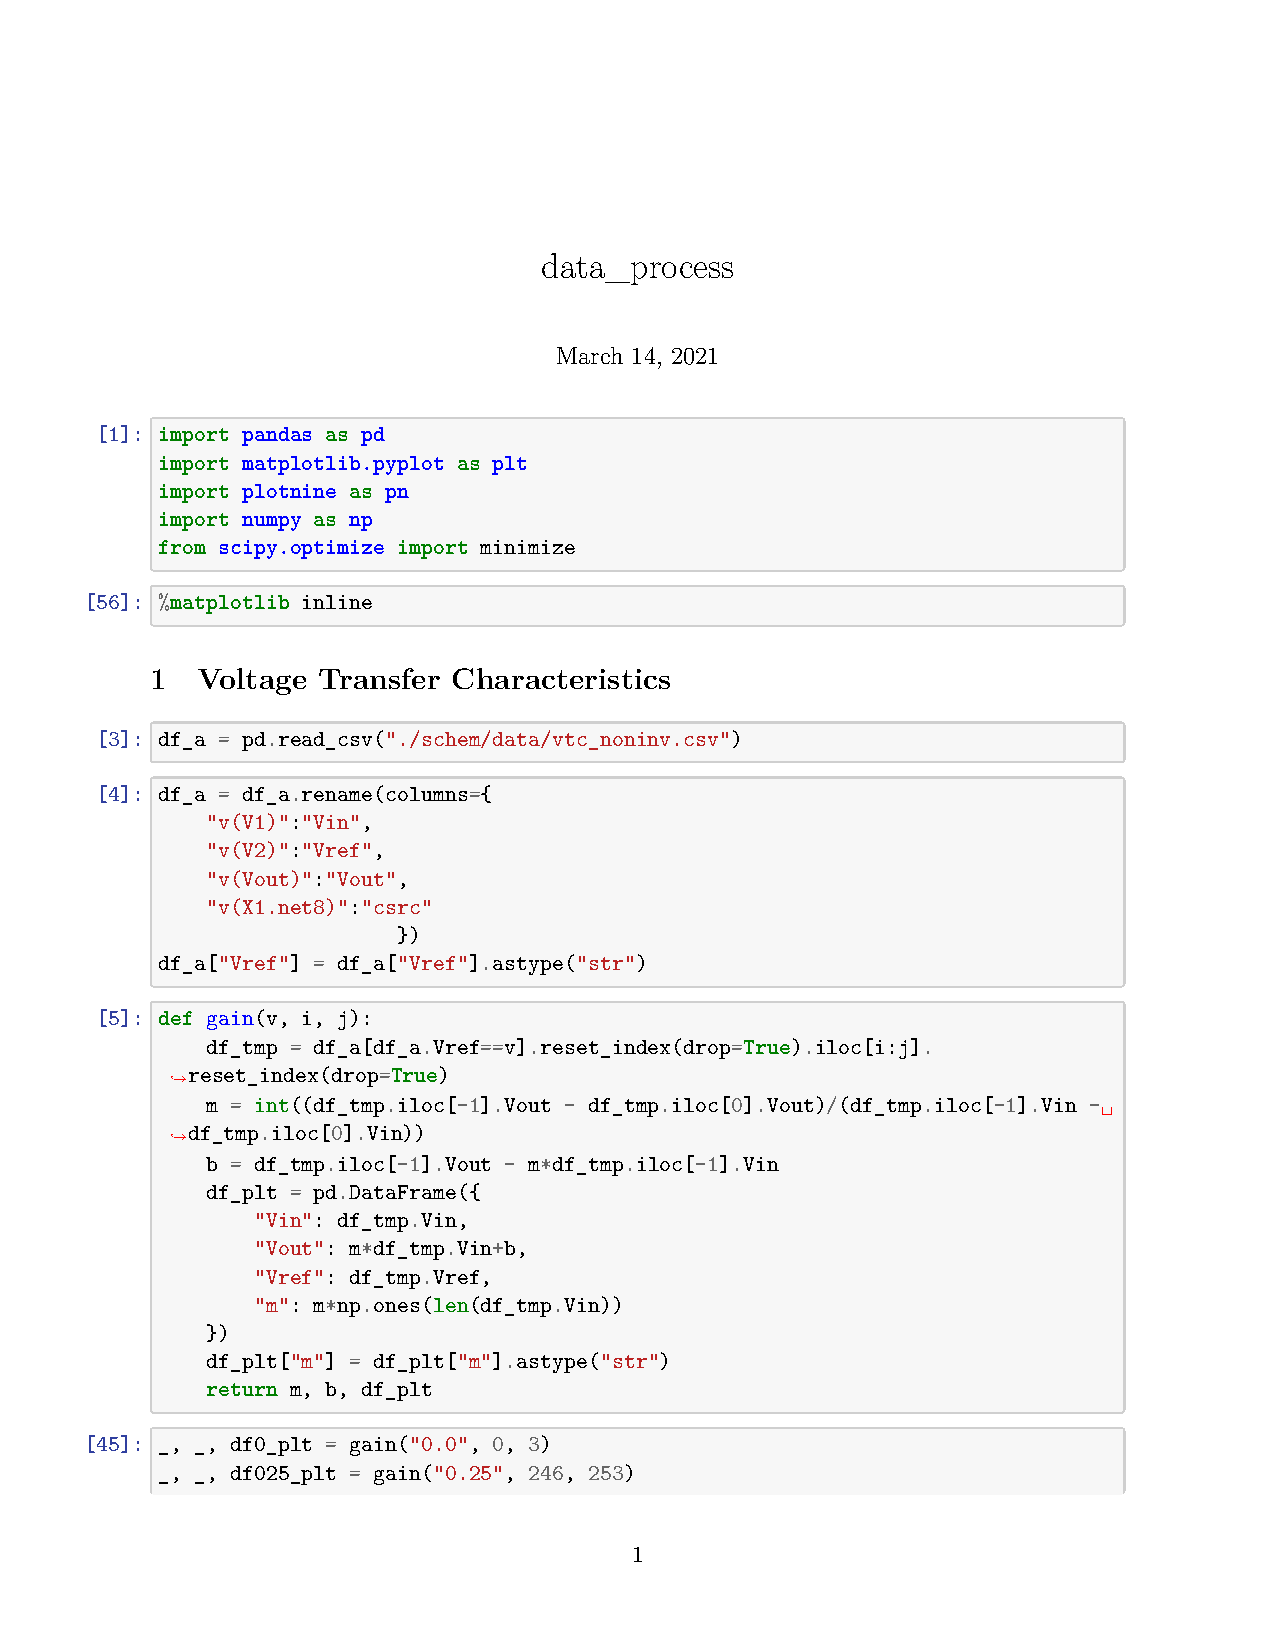
\includepdf[pages=-]{data_process.pdf}
\end{document}
